% Generated by thesis/ch7/exp1/networks.py -- do not edit by hand.
% Appendix: Experiment 1 networks, as trained and as explained.
% Picture height: 0.9 of the portrait text width, fixed here (inside a sidewaysfigure \textwidth is the
% page's long side).
\ifdefined\netfigheight\else\newlength{\netfigheight}\setlength{\netfigheight}{0.9\textwidth}\fi
% Spreads: a case's heading on a right (odd) page, its raw network on the left (even) page after it and
% the explained network facing it on the right.
\providecommand{\cleartoevenpage}{\clearpage\ifodd\value{page}\hbox{}\thispagestyle{empty}\newpage\fi}
\providecommand{\cleartooddpage}{\clearpage\ifodd\value{page}\else\hbox{}\thispagestyle{empty}\newpage\fi}
\section{Experiment 1 networks}\label{app:exp1-networks}
% Adult, original network
\cleartooddpage
\subsection{Adult}\label{app:exp1-net-adult}
\cleartoevenpage
\begin{sidewaysfigure}
  \centering
  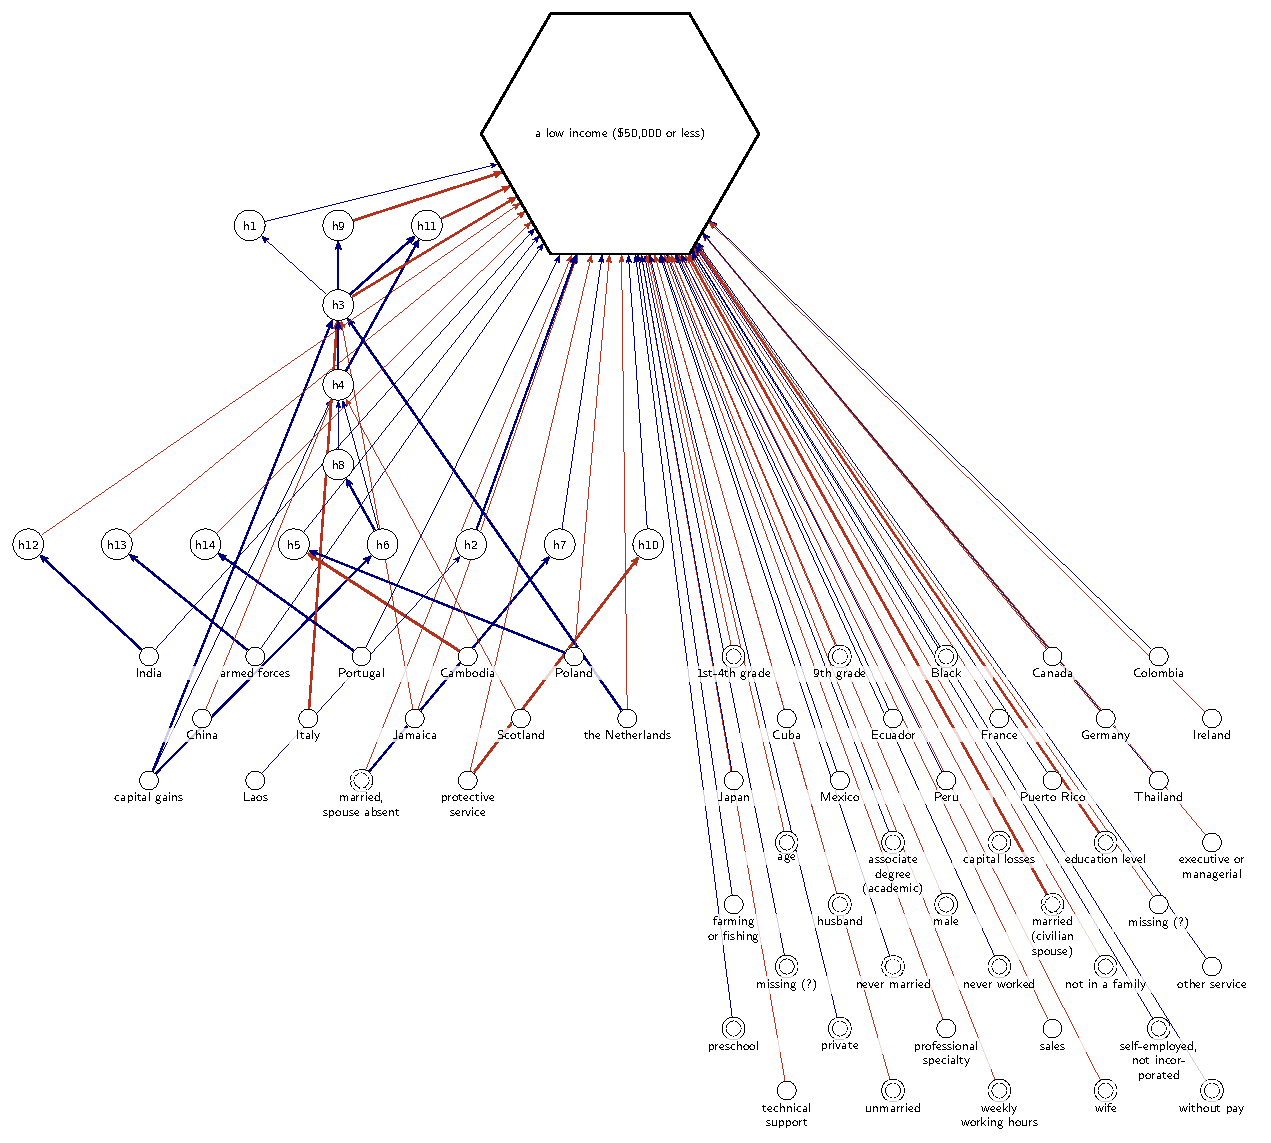
\includegraphics[width=\textheight,height=\netfigheight,keepaspectratio]{figures/exp1/networks/paper-adult-raw}
  \caption{Adult, original network: the network as trained, before any explanation. Bottom: the input columns; circles h1, h2, \ldots: hidden units; hexagon: the output. Edges: blue, a positive weight (raises the score); red, a negative weight (lowers it); thicker, a larger weight. Double outline: acts at a fixed rate everywhere (dashed double: on the observed data).}
  \label{fig:exp1-net-paper-adult-raw}
\end{sidewaysfigure}
\clearpage
\begin{sidewaysfigure}
  \centering
  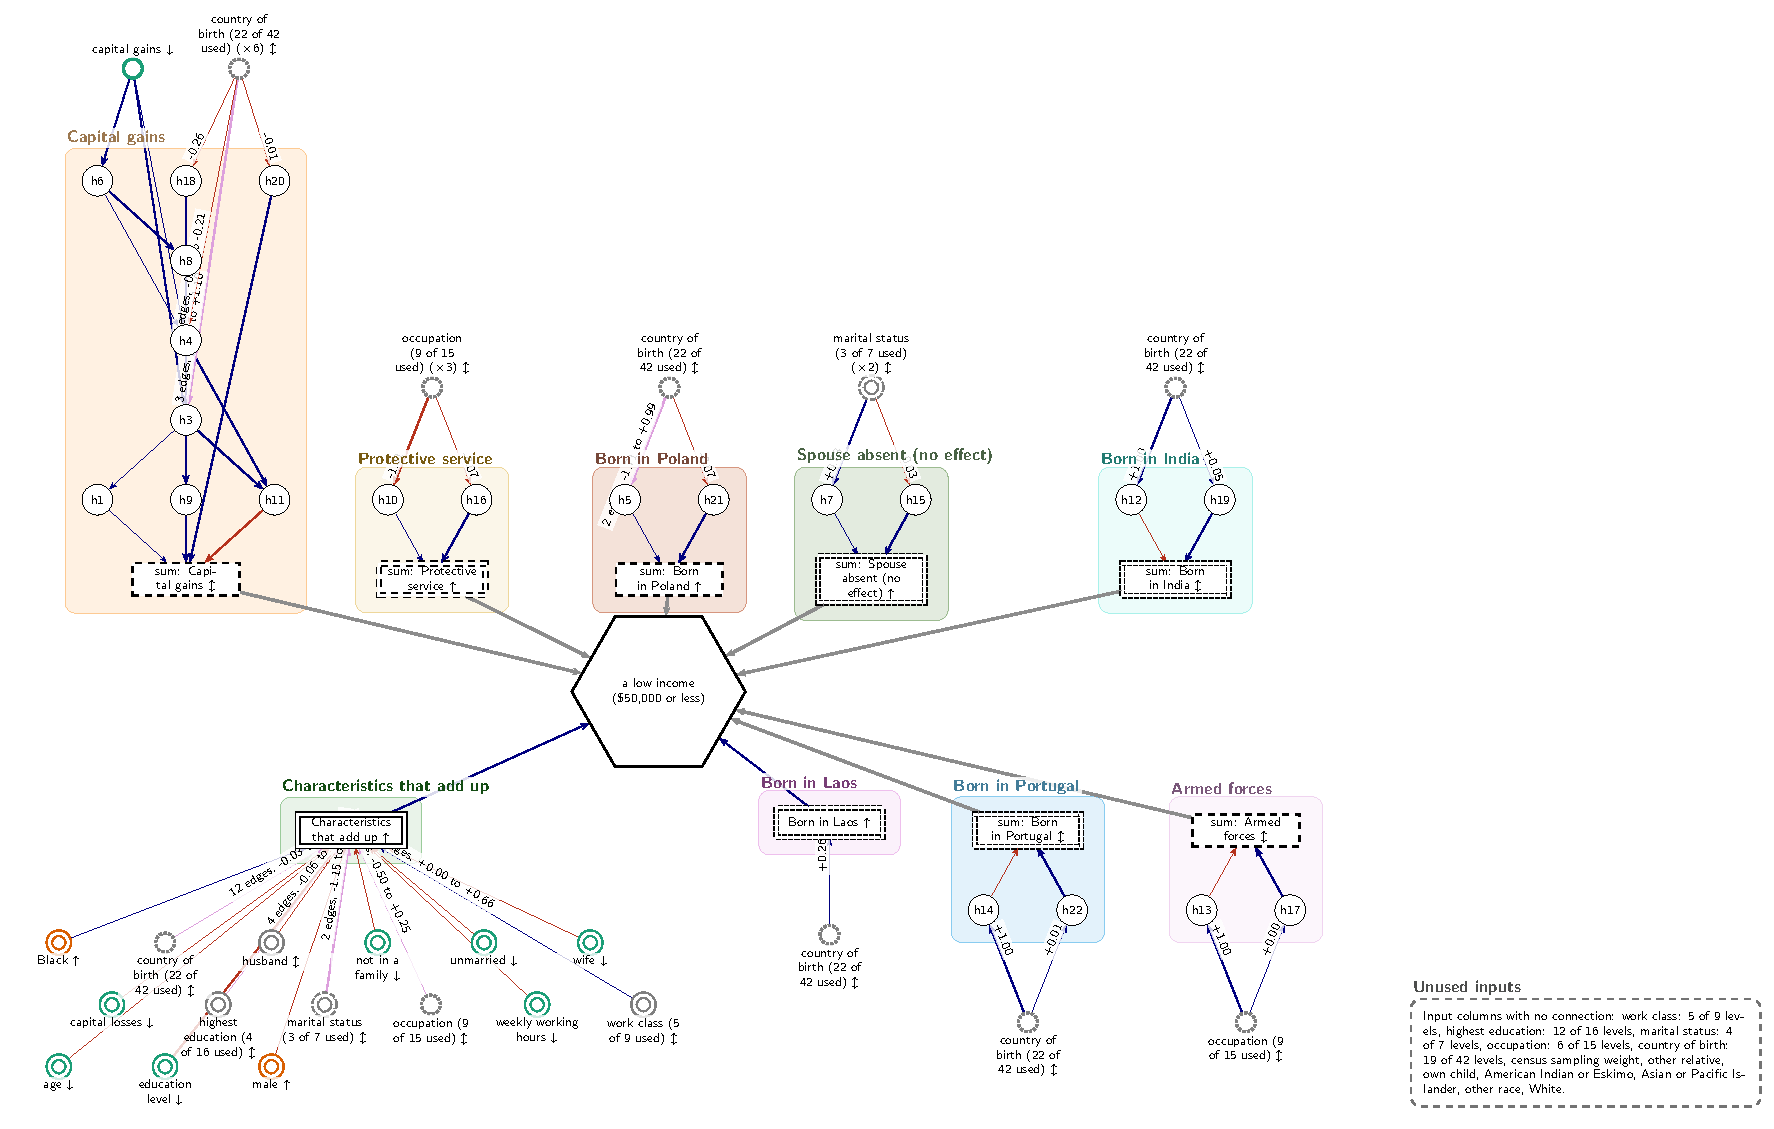
\includegraphics[width=\textheight,height=\netfigheight,keepaspectratio]{figures/exp1/networks/paper-adult-explained}
  \caption{Adult, original network: the explained network, every unit nested by part. Shaded boxes: the explanation's parts (inner boxes: sub-parts); white box: a part's output (dashed: a sum standing for the output unit's addition, grey edge). Each input is drawn under every part that reads it (dotted outline, $\times n$: read by $n$ parts); a variable with many levels is drawn once, its edges labelled with their number and weight range (purple: both signs). Orange outline and up arrow: raises the final prediction; teal and down arrow: lowers it; grey and double arrow: depends. Double outline: acts at a fixed rate everywhere (dashed double: on the observed data). Edges as in Figure~\ref{fig:exp1-net-paper-adult-raw}. Dashed grey box, right: the annotation of the input columns with no connection, outside the root.}
  \label{fig:exp1-net-paper-adult-explained}
\end{sidewaysfigure}
\clearpage
\clearpage
% Heart, original network
\cleartooddpage
\subsection{Heart}\label{app:exp1-net-heart}
\cleartoevenpage
\begin{sidewaysfigure}
  \centering
  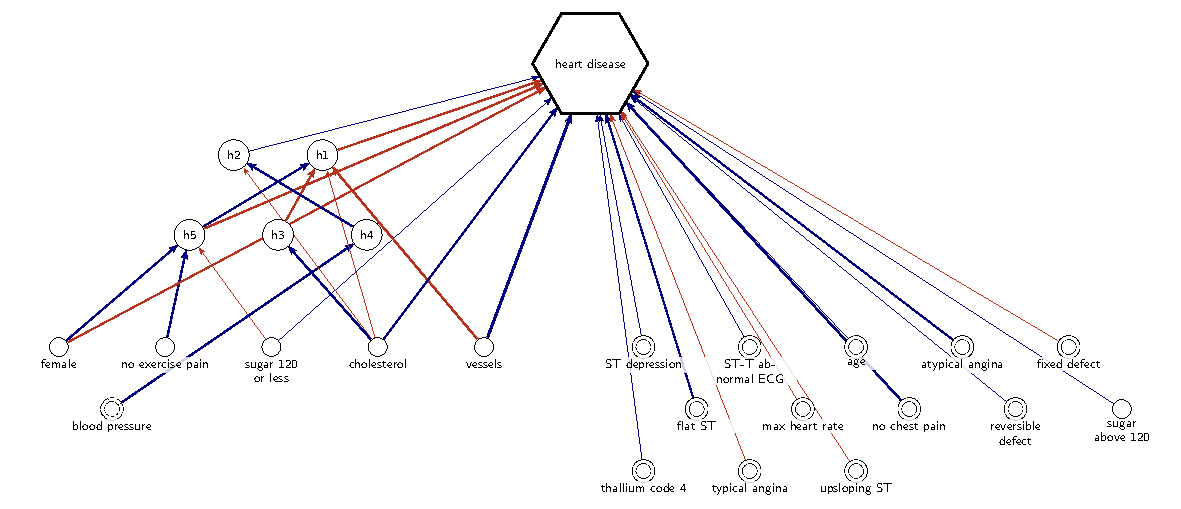
\includegraphics[width=\textheight,height=\netfigheight,keepaspectratio]{figures/exp1/networks/paper-heart-raw}
  \caption{Heart, original network: the network as trained, before any explanation. Bottom: the input columns; circles h1, h2, \ldots: hidden units; hexagon: the output. Edges: blue, a positive weight (raises the score); red, a negative weight (lowers it); thicker, a larger weight. Double outline: acts at a fixed rate everywhere (dashed double: on the observed data).}
  \label{fig:exp1-net-paper-heart-raw}
\end{sidewaysfigure}
\clearpage
\begin{sidewaysfigure}
  \centering
  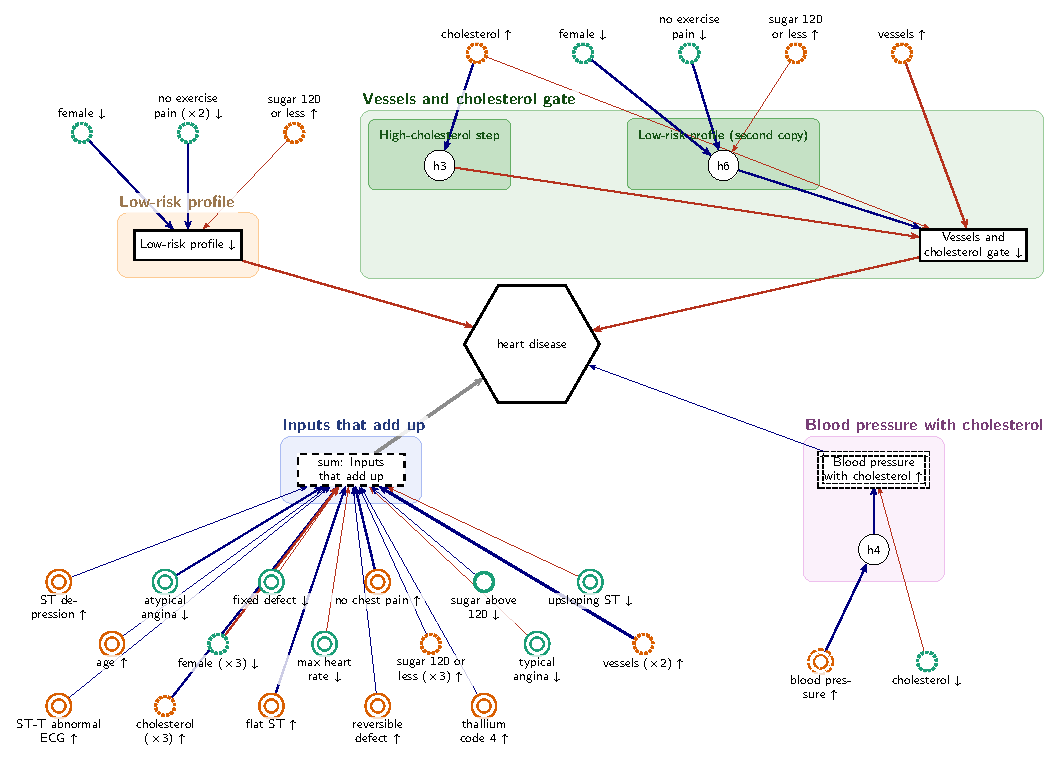
\includegraphics[width=\textheight,height=\netfigheight,keepaspectratio]{figures/exp1/networks/paper-heart-explained}
  \caption{Heart, original network: the explained network, every unit nested by part. Shaded boxes: the explanation's parts (inner boxes: sub-parts); white box: a part's output (dashed: a sum standing for the output unit's addition, grey edge). Each input is drawn under every part that reads it (dotted outline, $\times n$: read by $n$ parts); a variable with many levels is drawn once, its edges labelled with their number and weight range (purple: both signs). Orange outline and up arrow: raises the final prediction; teal and down arrow: lowers it; grey and double arrow: depends. Double outline: acts at a fixed rate everywhere (dashed double: on the observed data). Edges as in Figure~\ref{fig:exp1-net-paper-heart-raw}.}
  \label{fig:exp1-net-paper-heart-explained}
\end{sidewaysfigure}
\clearpage
\clearpage
% MONK-2, original network
\cleartooddpage
\subsection{MONK-2}\label{app:exp1-net-monk2}
\cleartoevenpage
\begin{sidewaysfigure}
  \centering
  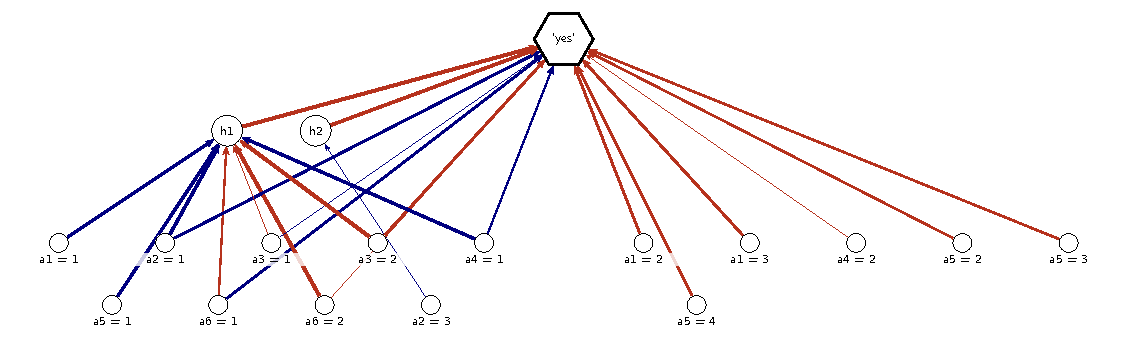
\includegraphics[width=\textheight,height=\netfigheight,keepaspectratio]{figures/exp1/networks/paper-monk2-raw}
  \caption{MONK-2, original network: the network as trained, before any explanation. Bottom: the input columns; circles h1, h2, \ldots: hidden units; hexagon: the output. Edges: blue, a positive weight (raises the score); red, a negative weight (lowers it); thicker, a larger weight. Double outline: acts at a fixed rate everywhere (dashed double: on the observed data).}
  \label{fig:exp1-net-paper-monk2-raw}
\end{sidewaysfigure}
\clearpage
\begin{sidewaysfigure}
  \centering
  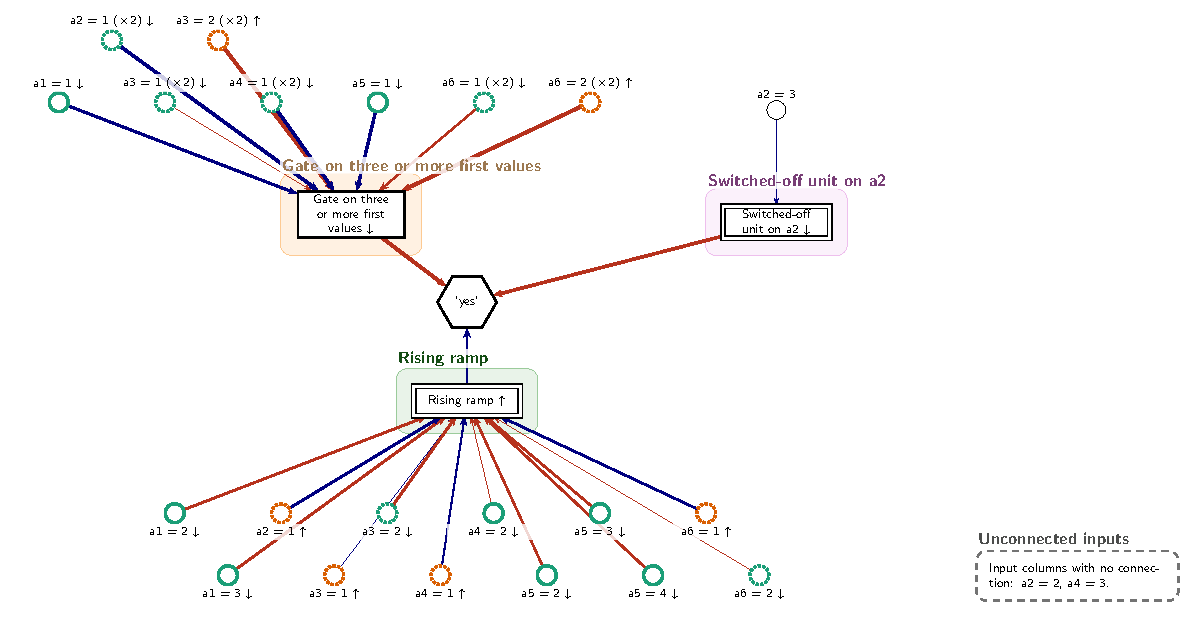
\includegraphics[width=\textheight,height=\netfigheight,keepaspectratio]{figures/exp1/networks/paper-monk2-explained}
  \caption{MONK-2, original network: the explained network, every unit nested by part. Shaded boxes: the explanation's parts (inner boxes: sub-parts); white box: a part's output (dashed: a sum standing for the output unit's addition, grey edge). Each input is drawn under every part that reads it (dotted outline, $\times n$: read by $n$ parts); a variable with many levels is drawn once, its edges labelled with their number and weight range (purple: both signs). Orange outline and up arrow: raises the final prediction; teal and down arrow: lowers it; grey and double arrow: depends. Double outline: acts at a fixed rate everywhere (dashed double: on the observed data). Edges as in Figure~\ref{fig:exp1-net-paper-monk2-raw}. Dashed grey box, right: the annotation of the input columns with no connection, outside the root.}
  \label{fig:exp1-net-paper-monk2-explained}
\end{sidewaysfigure}
\clearpage
\clearpage
% Churn, seed 10
\cleartooddpage
\subsection{Churn}\label{app:exp1-net-churn}
\cleartoevenpage
\begin{sidewaysfigure}
  \centering
  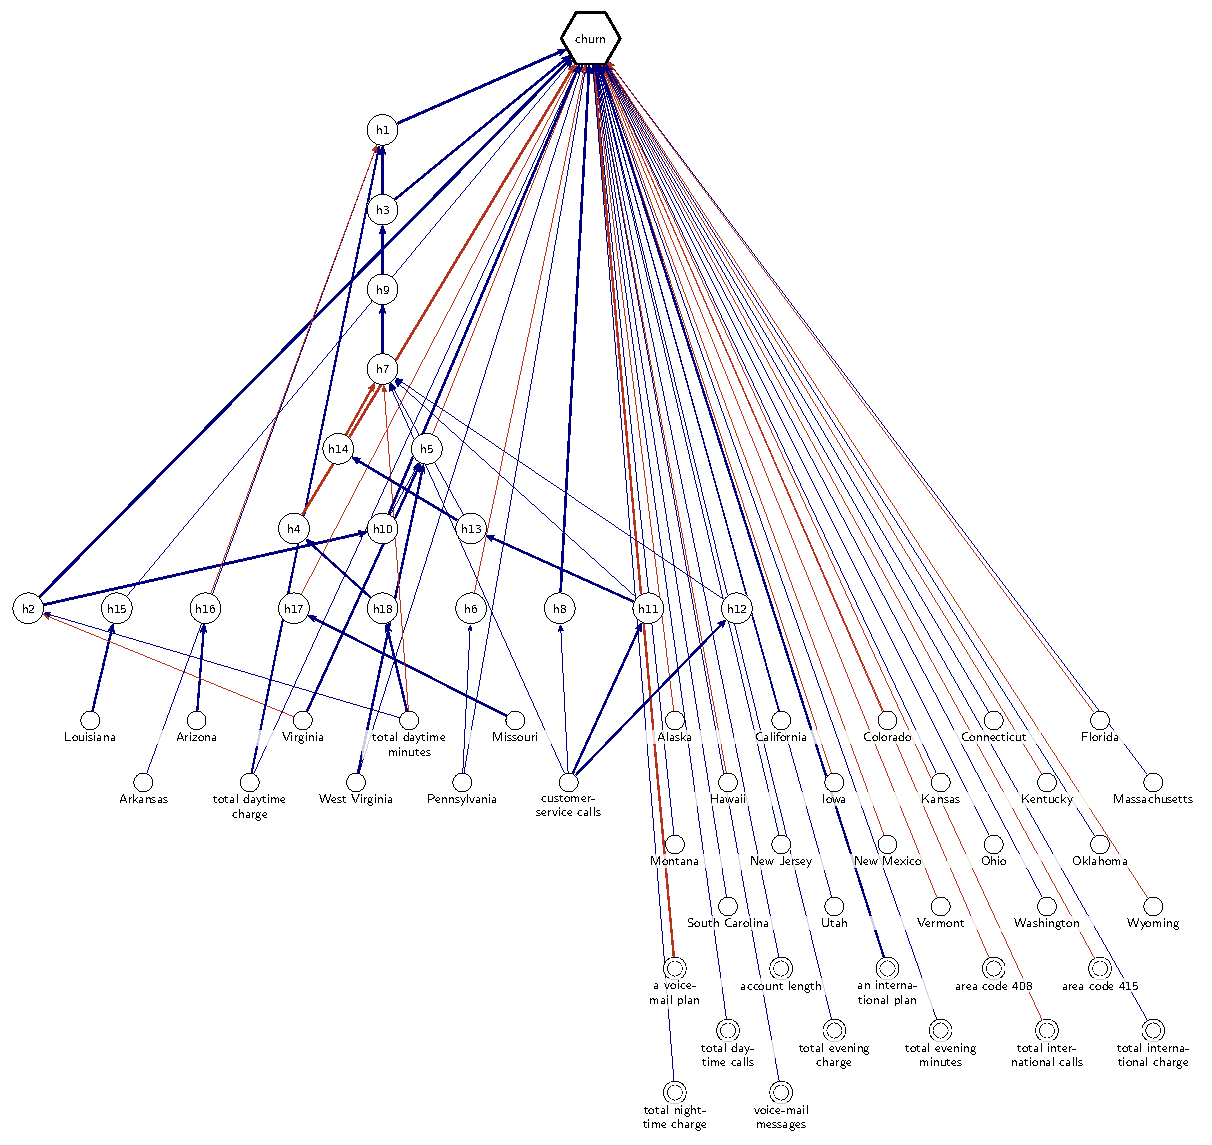
\includegraphics[width=\textheight,height=\netfigheight,keepaspectratio]{figures/exp1/networks/churn-case-s10-raw}
  \caption{Churn, seed 10: the network as trained, before any explanation. Bottom: the input columns; circles h1, h2, \ldots: hidden units; hexagon: the output. Edges: blue, a positive weight (raises the score); red, a negative weight (lowers it); thicker, a larger weight. Double outline: acts at a fixed rate everywhere (dashed double: on the observed data).}
  \label{fig:exp1-net-churn-case-s10-raw}
\end{sidewaysfigure}
\clearpage
\begin{sidewaysfigure}
  \centering
  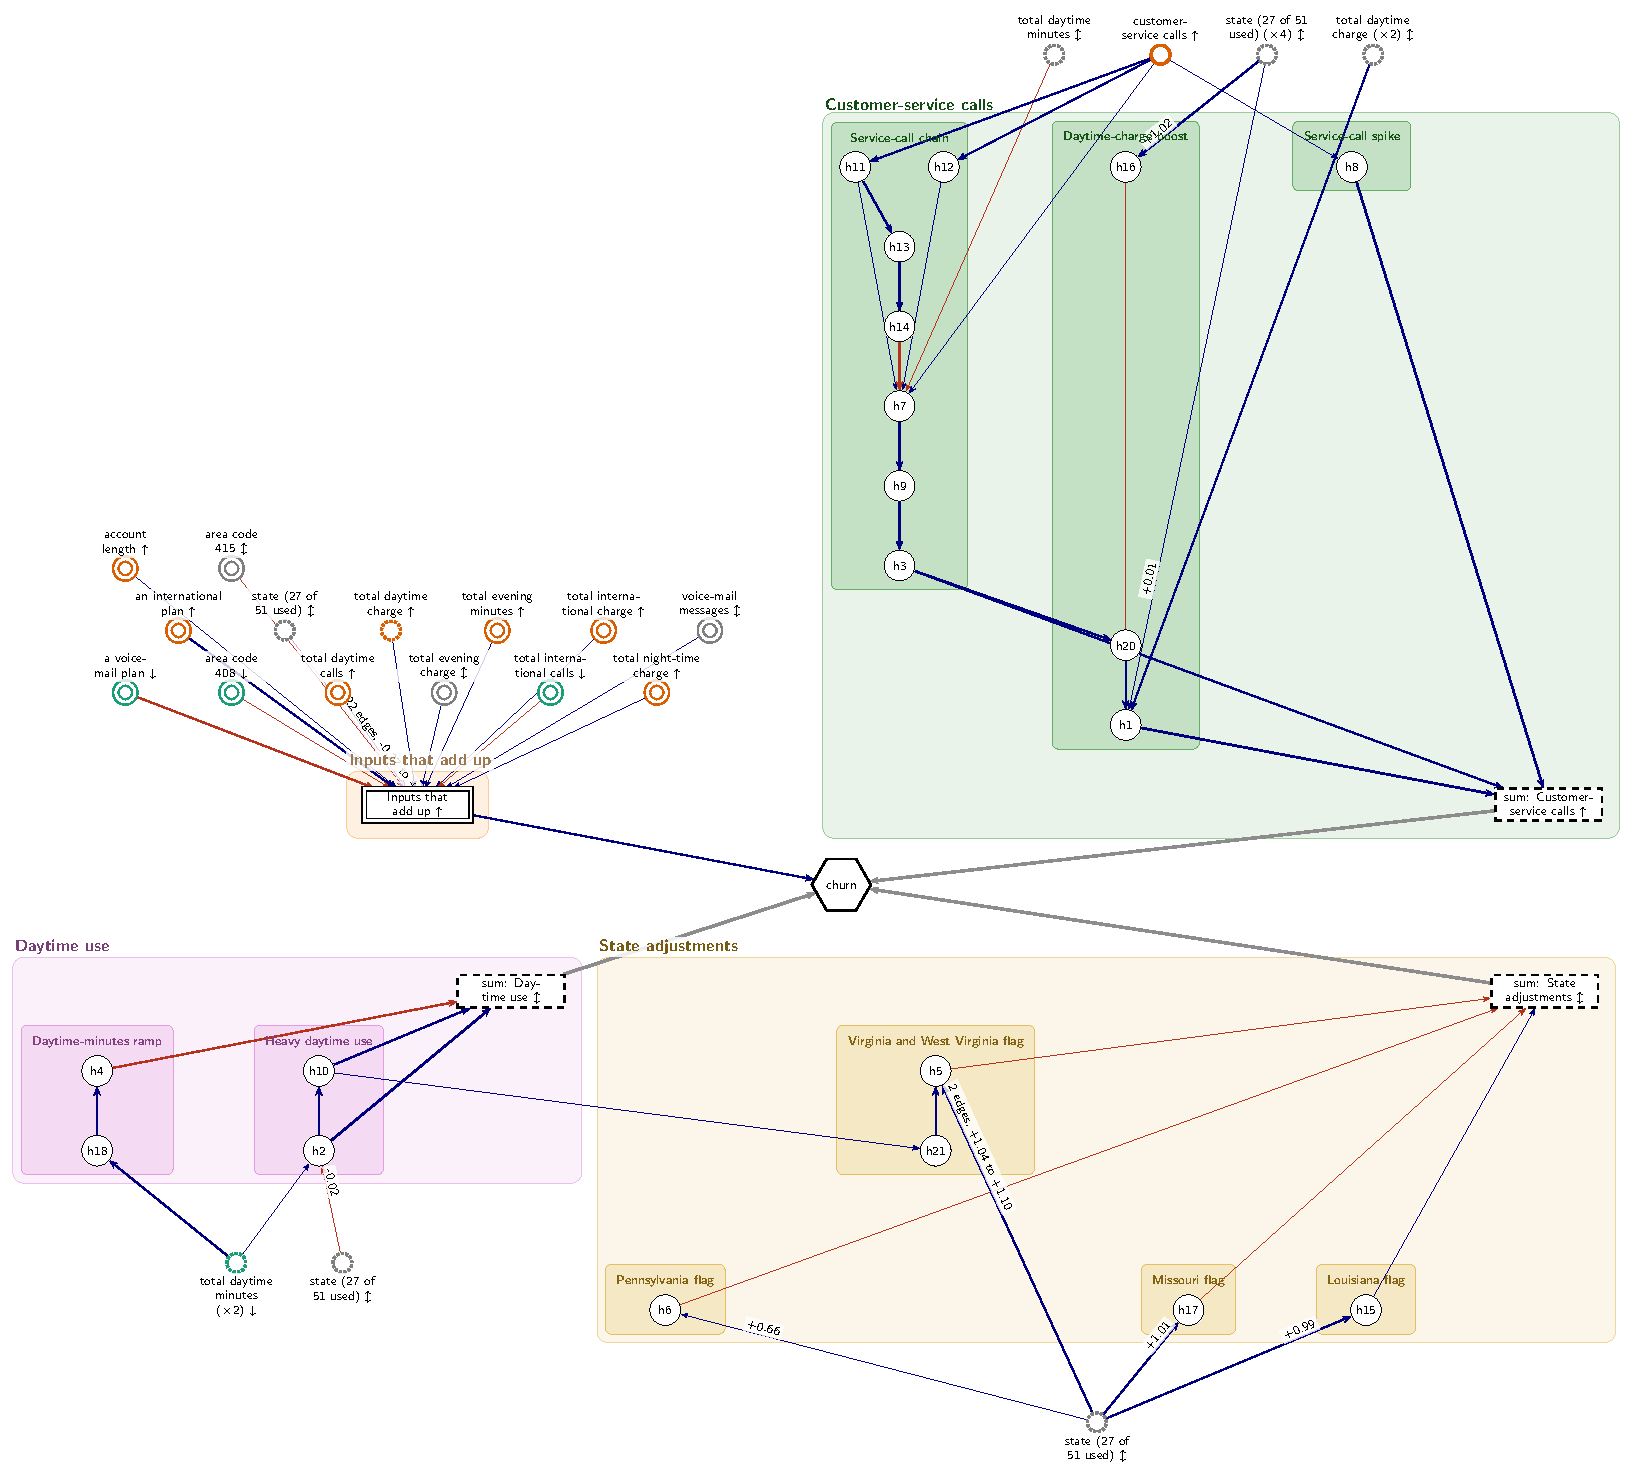
\includegraphics[width=\textheight,height=\netfigheight,keepaspectratio]{figures/exp1/networks/churn-case-s10-explained}
  \caption{Churn, seed 10: the explained network, every unit nested by part. Shaded boxes: the explanation's parts (inner boxes: sub-parts); white box: a part's output (dashed: a sum standing for the output unit's addition, grey edge). Each input is drawn under every part that reads it (dotted outline, $\times n$: read by $n$ parts); a variable with many levels is drawn once, its edges labelled with their number and weight range (purple: both signs). Orange outline and up arrow: raises the final prediction; teal and down arrow: lowers it; grey and double arrow: depends. Double outline: acts at a fixed rate everywhere (dashed double: on the observed data). Edges as in Figure~\ref{fig:exp1-net-churn-case-s10-raw}.}
  \label{fig:exp1-net-churn-case-s10-explained}
\end{sidewaysfigure}
\clearpage
\clearpage
% Connect-4, cells, seed 1
\cleartooddpage
\subsection{Connect-4, cells}\label{app:exp1-net-c4cells}
\begin{sidewaysfigure}
  \centering
  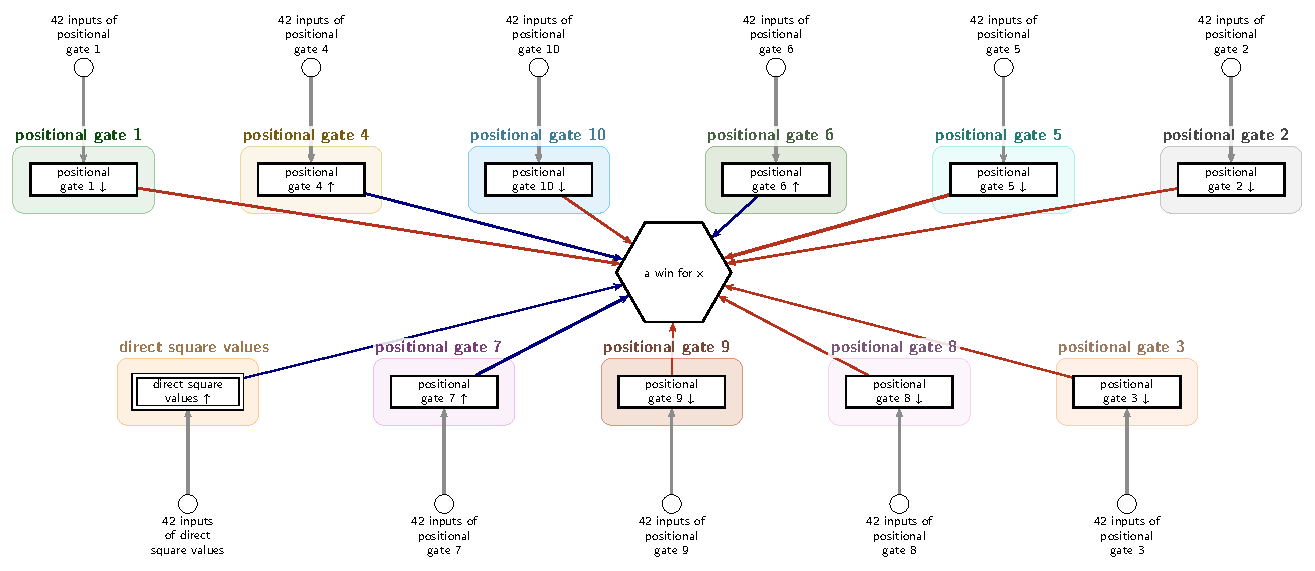
\includegraphics[width=\textheight,height=\netfigheight,keepaspectratio]{figures/exp1/networks/c4cap-main-h10-e50-s1-explained}
  \caption{Connect-4, cells, seed 1: the explained network, each top-level part collapsed into one box (its output), the inputs each part reads below it. Grey edges: the inputs a collapsed part reads (no single weight); a part reading many input columns has them drawn as one input. Arrows on inputs and boxes: the direction of the effect on the final prediction (up raises it, down lowers it, double arrow depends). Edges: blue, a positive weight (raises the score); red, a negative weight (lowers it); thicker, a larger weight.}
  \label{fig:exp1-net-c4cap-main-h10-e50-s1-explained}
\end{sidewaysfigure}
\clearpage
\clearpage
% Connect-4, lines, seed 0
\cleartooddpage
\subsection{Connect-4, lines}\label{app:exp1-net-c4lines}
\cleartoevenpage
\begin{sidewaysfigure}
  \centering
  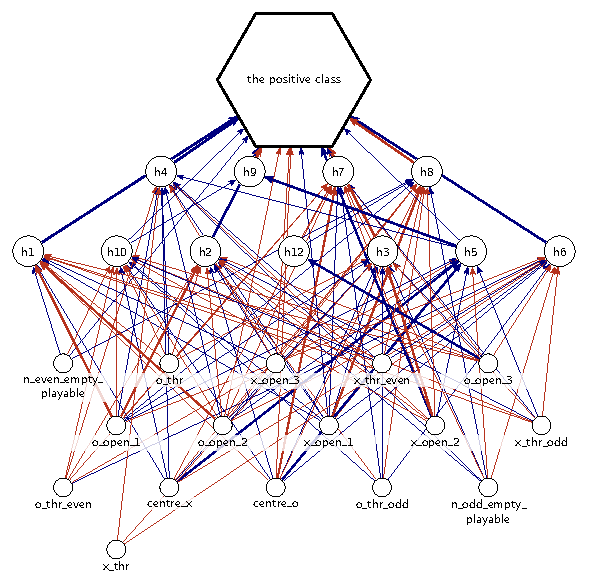
\includegraphics[width=\textheight,height=\netfigheight,keepaspectratio]{figures/exp1/networks/c4lf-lines-heavy-s0-raw}
  \caption{Connect-4, lines, seed 0: the network as trained, before any explanation. Bottom: the input columns; circles h1, h2, \ldots: hidden units; hexagon: the output. Edges: blue, a positive weight (raises the score); red, a negative weight (lowers it); thicker, a larger weight. Double outline: acts at a fixed rate everywhere (dashed double: on the observed data).}
  \label{fig:exp1-net-c4lf-lines-heavy-s0-raw}
\end{sidewaysfigure}
\clearpage
\begin{sidewaysfigure}
  \centering
  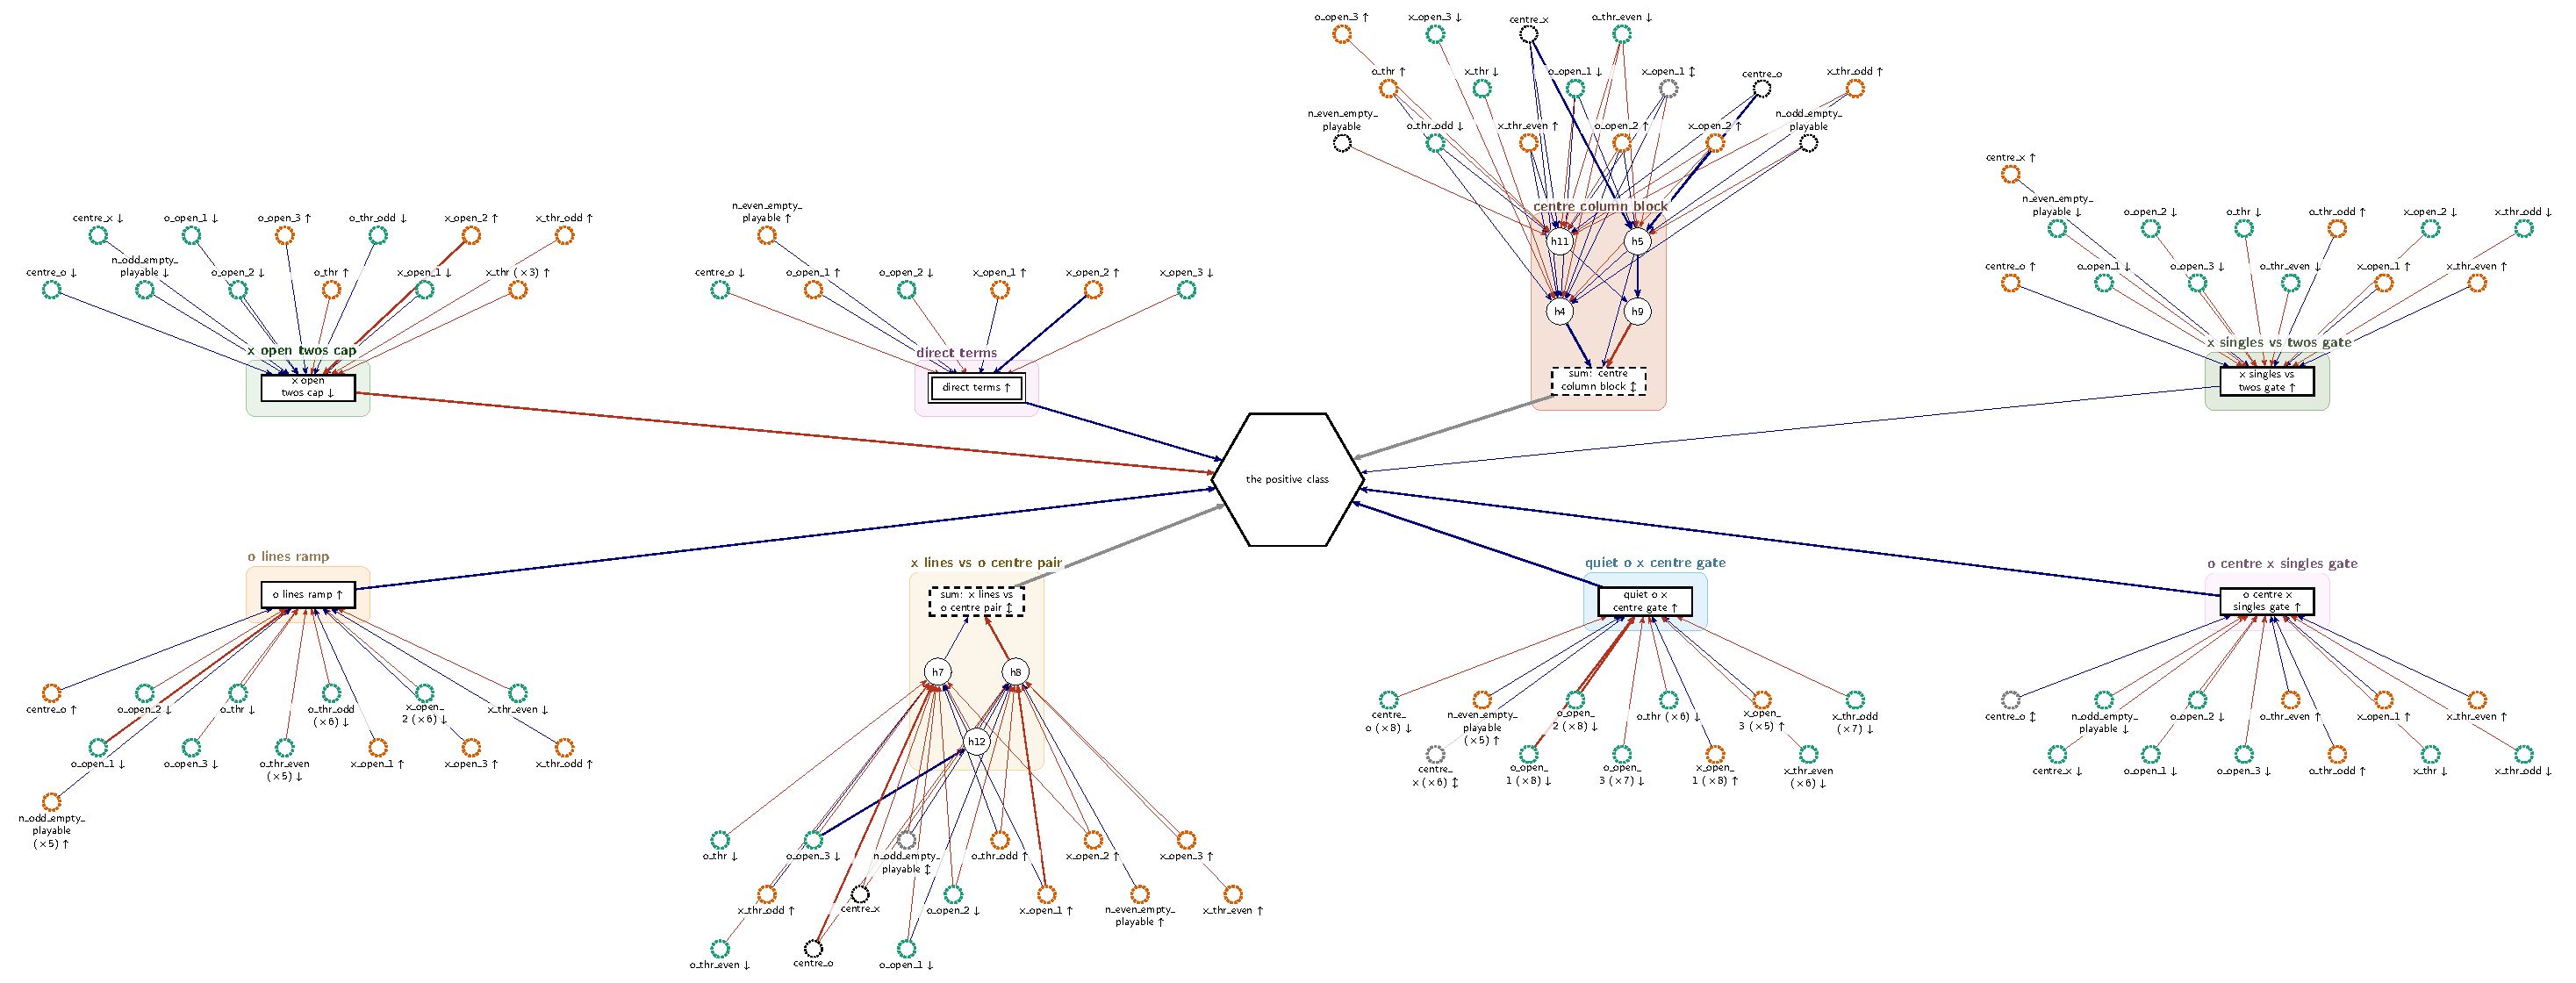
\includegraphics[width=\textheight,height=\netfigheight,keepaspectratio]{figures/exp1/networks/c4lf-lines-heavy-s0-explained}
  \caption{Connect-4, lines, seed 0: the explained network, each top-level part collapsed into one box (its output), the inputs each part reads below it. Grey edges: the inputs a collapsed part reads (no single weight); a part reading many input columns has them drawn as one input. Arrows on inputs and boxes: the direction of the effect on the final prediction (up raises it, down lowers it, double arrow depends). Edges: blue, a positive weight (raises the score); red, a negative weight (lowers it); thicker, a larger weight.}
  \label{fig:exp1-net-c4lf-lines-heavy-s0-explained}
\end{sidewaysfigure}
\clearpage
\clearpage
% Synthetic U and saddle, seed 4
\cleartooddpage
\subsection{Synthetic U and saddle}\label{app:exp1-net-shapeC}
\cleartoevenpage
\begin{sidewaysfigure}
  \centering
  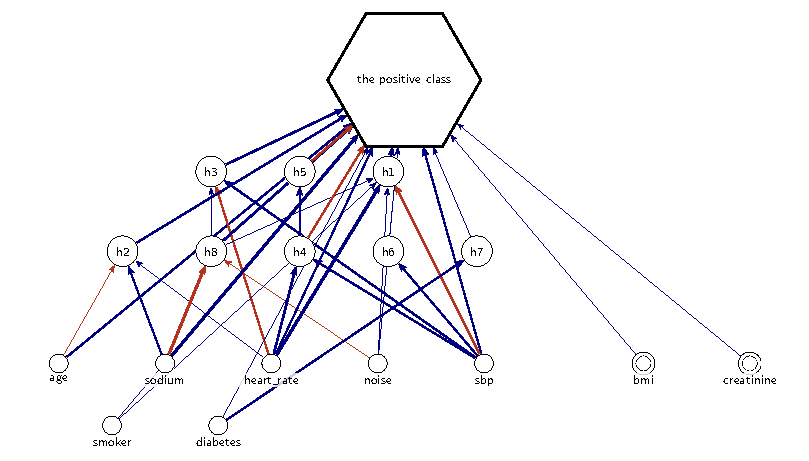
\includegraphics[width=\textheight,height=\netfigheight,keepaspectratio]{figures/exp1/networks/shape-C-raw}
  \caption{Synthetic U and saddle, seed 4: the network as trained, before any explanation. Bottom: the input columns; circles h1, h2, \ldots: hidden units; hexagon: the output. Edges: blue, a positive weight (raises the score); red, a negative weight (lowers it); thicker, a larger weight. Double outline: acts at a fixed rate everywhere (dashed double: on the observed data).}
  \label{fig:exp1-net-shape-C-raw}
\end{sidewaysfigure}
\clearpage
\begin{sidewaysfigure}
  \centering
  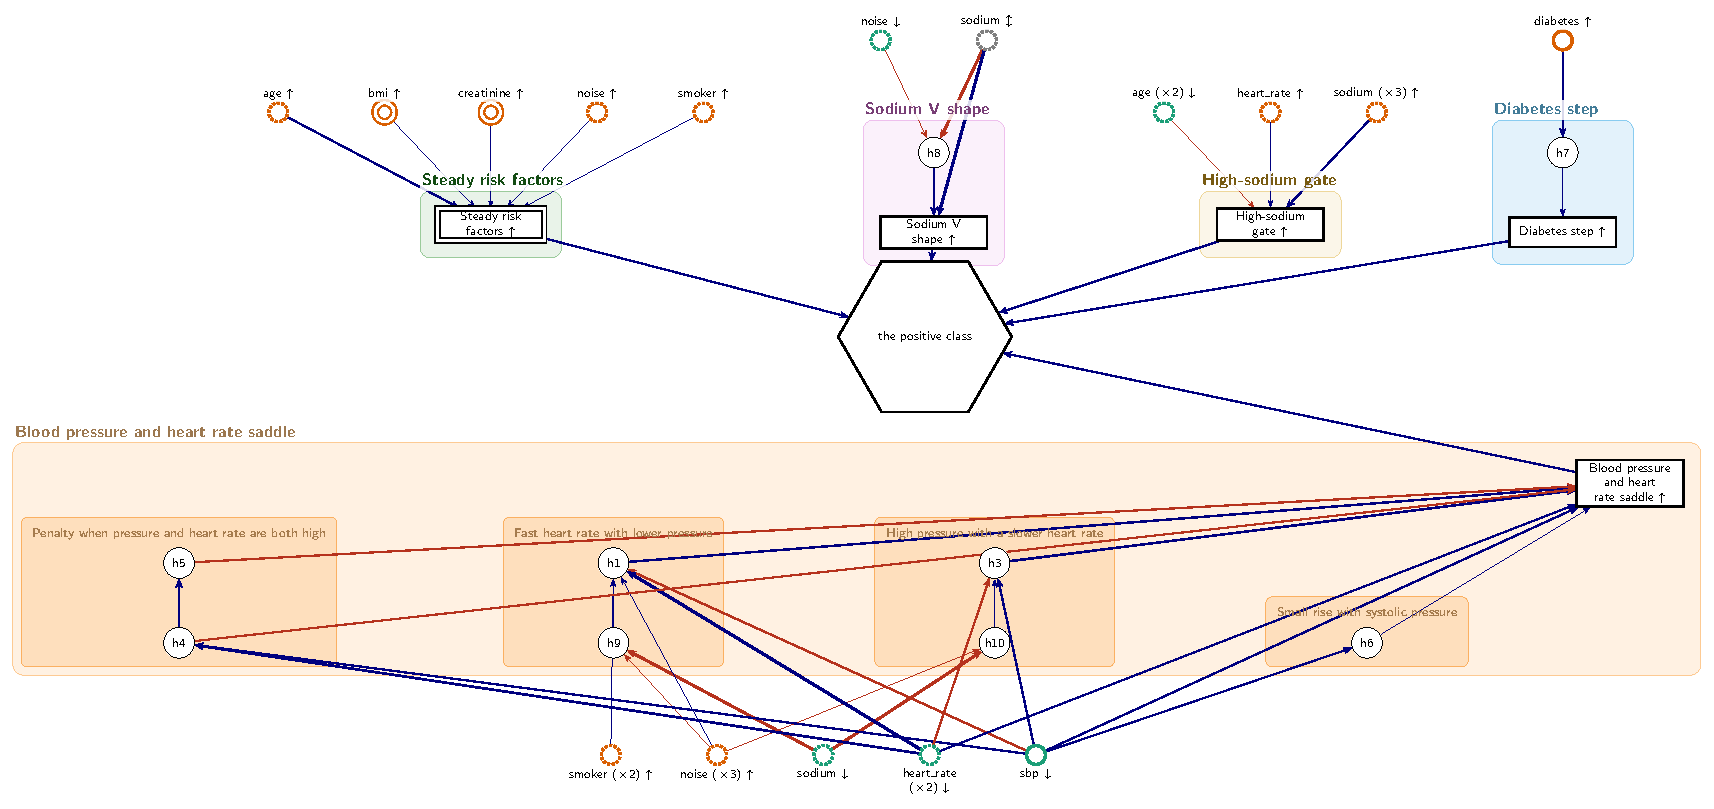
\includegraphics[width=\textheight,height=\netfigheight,keepaspectratio]{figures/exp1/networks/shape-C-explained}
  \caption{Synthetic U and saddle, seed 4: the explained network, every unit nested by part. Shaded boxes: the explanation's parts (inner boxes: sub-parts); white box: a part's output (dashed: a sum standing for the output unit's addition, grey edge). Each input is drawn under every part that reads it (dotted outline, $\times n$: read by $n$ parts); a variable with many levels is drawn once, its edges labelled with their number and weight range (purple: both signs). Orange outline and up arrow: raises the final prediction; teal and down arrow: lowers it; grey and double arrow: depends. Double outline: acts at a fixed rate everywhere (dashed double: on the observed data). Edges as in Figure~\ref{fig:exp1-net-shape-C-raw}.}
  \label{fig:exp1-net-shape-C-explained}
\end{sidewaysfigure}
\clearpage
\clearpage
% XOR
\cleartooddpage
\subsection{XOR}\label{app:exp1-net-xor}
\begin{figure}[!htbp]
  \centering
  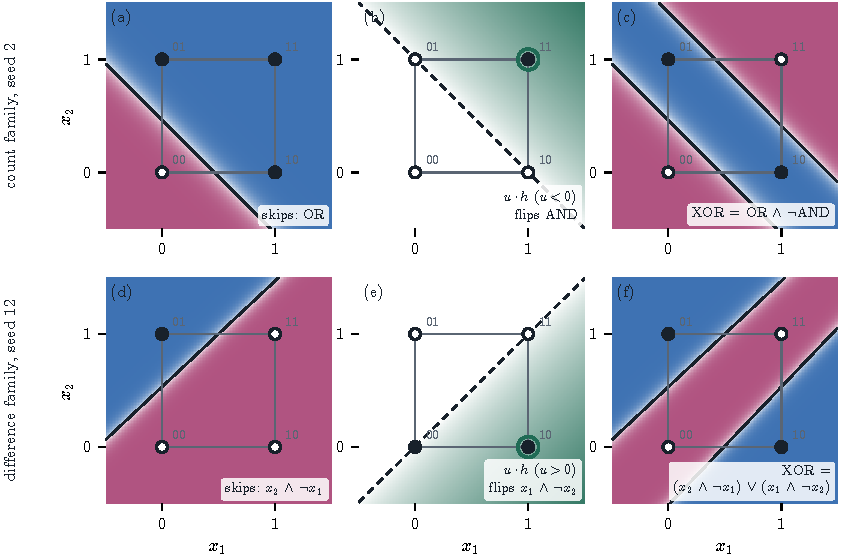
\includegraphics[width=\textwidth,height=0.8\textheight,keepaspectratio]{figures/ch7/xor-gates.pdf}
  \caption{XOR: the gates of the networks of Figure~\ref{fig:ch7-xor-ridge-valley}, the count family (a--c; seed 2) and the difference family (d--f; seed 12). Left: the skip connections alone; middle: the hidden unit's contribution $u\cdot h$ (green: active, darker for larger $|u h|$; dashed: its fold; ringed points: the inputs whose sign it flips); right: the composed score. Shading: blue where the score is positive, magenta where it is negative, pale near 0; solid line: where it is 0. Filled points: inputs where the panel's quantity is positive (middle: where the hidden unit is active).}
  \label{fig:ch7-xor-gates}
\end{figure}
\begin{figure}[!htbp]
  \centering
  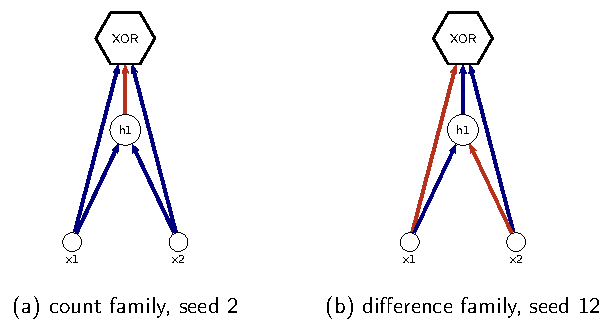
\includegraphics[width=\textwidth,height=0.8\textheight,keepaspectratio]{figures/exp1/networks/xor-raw}
  \caption{XOR: one minimal network of each family, reduced, before any explanation. (a) Count family; (b) difference family. Bottom: the input columns; circles h1, h2, \ldots: hidden units; hexagon: the output. Edges: blue, a positive weight (raises the score); red, a negative weight (lowers it); thicker, a larger weight.}
  \label{fig:exp1-net-xor-raw}
\end{figure}
\clearpage
